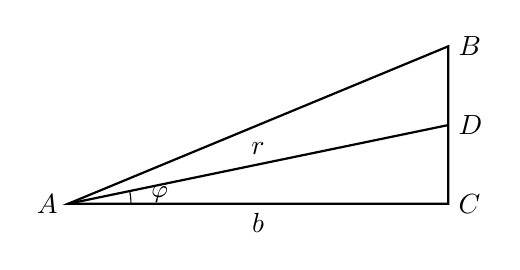
\begin{tikzpicture}
  \def \a {4}
  \def \b {(\a/2 + \a/sqrt(2))}

  \coordinate (A) at (0, 0);
  \coordinate (B) at ({\b}, {\a/2});
  \coordinate (C) at ({\b}, 0);
  \coordinate (D) at ({\b}, {\a/4});

  \draw[thick] (A) node[anchor=east] {$A$}
    -- (B) node[anchor=west] {$B$} 
    -- (C) node[anchor=west] {$C$} 
    -- cycle;

  \draw (A) -- (C) node[midway, anchor=north] {$b$};
  \draw[thick] (A) -- (D) node[midway, anchor=south] {$r$}
                          node[anchor=west] {$D$};

  \draw (0.8, 0) arc (0:{atan((\a/2/2)/\b)}:0.8) node[midway, anchor=west, xshift=4, yshift=1] {\small{$\varphi$}};
\end{tikzpicture}
